\subsection{Local Search by Simulated Annealing}
\label{sec:algo_ls}

We first build an IsA graph from the entities/concepts in each specific argument of a verb \footnote{This graph is actually a subgraph of the
Probase graph.}. As shown in \figref{fig:subgraph}, the graph is
a directed graph between the object instances of ``wear'' where each
arrow denotes an isA relation.
\begin{figure}[th]
\centering
\epsfig{file=subgraph.eps,width=0.5\columnwidth}
\caption{An IsA sub-graph for Objects of ``Wear''}
\label{fig:subgraph}
\end{figure}

Then, we propose a representative score to present how good a concept
is, by using Coverage and Inverse Typicality scores.
And below is the definition of  Coverage and Inverse Typicality:

\textbf{Coverage} - How much entities of the concept are covered by the local subgraph:
\begin{equation}
Cov(c) = \left\{ \begin{array}{ll}
1 & \textrm{, if $c \in L$}\\
\sum\limits_{e\in L}{P(e|c)=\sum\limits_{e\in L}{\frac{F(e,c)}{F(c)}}}& \textrm{, otherwise}
\end{array} \right.
\end{equation}
where $c$ is a concept, $L$ is the set of entities that appear in the local configuration, and $F(x)$ is the frequency of $x$ in Probase.

\textbf{Inverse Typicality} - How likely the concept to be the typical concept of the entities:
\begin{eqnarray}
IT(c)
&=& \frac{\sum_{e\in L}{P(e|L)P(c|e)+P(c|L)P(e|c)}}{\sum_{e\in L}{P(e|L)+\sum_{e_i}{P(c_i|L)P(e|c_i)}}} \nonumber\\
&=& \frac{\sum_{e\in L}{(F_l(e)\times \frac{F(e,c)}{F(e)}+F_l(c)\times \frac{F(e,c)}{F(c)})}}{\sum_{e\in L}{(F_l(e)+\sum_{c_i\in L}{F_l(c_i)\times \frac{F(e,c_i)}{F(c_i)}})}}
\end{eqnarray}
Where $F_l(x)$ is the local frequency of $x$. $L$ means the list of the objects of the given verb.

So the representative score of a concept $c$ is computed as follows:
\begin{equation}
RS(c) = Cov(c) \times IT(c)\times F_l(c)
\end{equation}

Because the action conceptualization problem is hard, we propose a
local search based approach here.
%This approach has two steps: Initialization by a greedy method and
%local search by Simulated Annealing.
%Next we discuss each step in detail.


%\subsubsection{Initialization}
%In order to get a good initial solution, we do the initialization process by a greedy method. Our algorithm first ranks the candidate concepts by representative score from largest to smallest. As in \secref{sec:greedy},
%our candidates are all those concepts in Probase which are in the
%input arguments.
%We then select the concepts one by one according to the ranking above
%as long as they satisfy the overlap constraint among the selected
%concepts, until all the arguments in the input are covered.
%Details is shown in Algorithm \ref{initialization}.
%\begin{algorithm}[th]
%\caption{Initialization by greedy method}
%\label{initialization}
%\begin{algorithmic}[1]
%\Function{CheckCover}{corpusE,conceptList}
%\State $flag \leftarrow true$
%\For{$e \in corpusE$}
%\State $flag' \leftarrow false$
%\For{$c \in conceptList$}
%\If{$e\ isA\ c$}
%\State $flag' \leftarrow true$, \textbf{break}
%\EndIf
%\EndFor
%\If{$flag'=false$}
%\State $flag \leftarrow false$, \textbf{break}
%\EndIf
%\EndFor
%\State \textbf{return} $flag$
%\EndFunction
%\Statex
%\Function{CheckOverlap}{$c_1$,$c_2$,overlapRate}
%\State $l_1 \leftarrow size(c_1)$, $l_2 \leftarrow size(c_2)$
%\State $l_{min} \leftarrow min(l_1,l_2)$, $sum \leftarrow 0$
%\If{$l_1 \leq l_2$}
%\For{$e \in entities\ of\ l_1$}
%\If{$e\ isA\ l_2$}
%\State $sum \leftarrow sum+1$
%\EndIf
%\EndFor
%\Else
%\For{$e \in entities\ of\ l_2$}
%\If{$e\ isA\ l_1$}
%\State $sum \leftarrow sum+1$
%\EndIf
%\EndFor
%\EndIf
%\If{$sum/l_{min} \leq overlapRate$}
%\State \textbf{return} $true$
%\Else
%\State \textbf{return} $false$
%\EndIf
%\EndFunction
%\Statex
%\Function{Initialization}{corpusE,candidateC,overlapRate}
%\State $initialC \leftarrow \emptyset$
%\State $rank\ candidateC\ by\ representative\ score$
%\For{$c \in candidateC$}
%\State $coverAll \leftarrow CheckCover(corpusE,initialC)$
%\If{$coverAll=true$}
%\State \textbf{break}
%\EndIf
%\State $flag \leftarrow true$
%\For{$c' \in initialC$}
%\State $overlap \leftarrow CheckOverlap(c,c',overlapRate)$
%\If{$overlap=false$}
%\State $flag \leftarrow false$, \textbf{break}
%\EndIf
%\EndFor
%\If{$flag=true$}
%\State $add\ c\ to\ initialC$
%\EndIf
%\EndFor
%\State \textbf{return} $initialC$
%\EndFunction
%\end{algorithmic}
%\end{algorithm}
%\begin{algorithm}[th]
%\caption{Initialization by greedy method}
%\label{initialization}
%\begin{algorithmic}[1]
%\Function{CheckCover}{corpusE,conceptList}
%\State $flag \leftarrow true$
%\For{$e \in corpusE$}
%\State $flag' \leftarrow false$
%\For{$c \in conceptList$}
%\If{$e\ isA\ c$}
%\State $flag' \leftarrow true$, \textbf{break}
%\EndIf
%\EndFor
%\If{$flag'=false$}
%\State $flag \leftarrow false$, \textbf{break}
%\EndIf
%\EndFor
%\State \textbf{return} $flag$
%\EndFunction
%\Statex
%\Function{CheckOverlap}{$c_1$,$c_2$,overlapRate}
%\State $l_1 \leftarrow size(c_1)$, $l_2 \leftarrow size(c_2)$
%\State $l_{min} \leftarrow min(l_1,l_2)$, $sum \leftarrow 0$
%\If{$l_1 \leq l_2$}
%\For{$e \in entities\ of\ l_1$}
%\If{$e\ isA\ l_2$}
%\State $sum \leftarrow sum+1$
%\EndIf
%\EndFor
%\Else
%\For{$e \in entities\ of\ l_2$}
%\If{$e\ isA\ l_1$}
%\State $sum \leftarrow sum+1$
%\EndIf
%\EndFor
%\EndIf
%\If{$sum/l_{min} \leq overlapRate$}
%\State \textbf{return} $true$
%\Else
%\State \textbf{return} $false$
%\EndIf
%\EndFunction
%\Statex
%\Function{Initialization}{corpusE,candidateC,overlapRate}
%\State $initialC \leftarrow \emptyset$
%\State $rank\ candidateC\ by\ representative\ score$
%\For{$c \in candidateC$}
%\State $coverAll \leftarrow CheckCover(corpusE,initialC)$
%\If{$coverAll=true$}
%\State \textbf{break}
%\EndIf
%\State $flag \leftarrow true$
%\For{$c' \in initialC$}
%\State $overlap \leftarrow CheckOverlap(c,c',overlapRate)$
%\If{$overlap=false$}
%\State $flag \leftarrow false$, \textbf{break}
%\EndIf
%\EndFor
%\If{$flag=true$}
%\State $add\ c\ to\ initialC$
%\EndIf
%\EndFor
%\State \textbf{return} $initialC$
%\EndFunction
%\end{algorithmic}
%\end{algorithm}

%\begin{algorithm}[th]
%\caption{Greedy Initialization}
%\label{initialization}
%\begin{algorithmic}[1]
%\Function{Initialization}{corpusE, candidateC, maxOverlap}
%\State $initialC \leftarrow \emptyset$
%\State rank $candidateC$ by representative score
%\For{$c \in candidateC$}
%\If{$candidateC$ can cover all entities in $corpusE$}
%\State \textbf{break}
%\EndIf
%\If{$c \cap c_i \le maxOverlap$ for all $c_i$ in $initialC$}
%\State add $c$ to $initialC$
%\EndIf
%\EndFor
%\State \textbf{return} $initialC$
%\EndFunction
%\end{algorithmic}
%\end{algorithm}

%As a special case, if some entities have no concept to cover, they can be selected as concepts without any overlap constraints.

We begin with initializing a candidate solution $initialC$
by greedily selecting top K concepts with largest representative score.
Then, in local search process, we first quantize the concept as follow:
$$
c_i =
\left[
\begin{array}{cccc}
p_{i1} & p_{i2} & \ldots & p_{in}
\end{array}
\right]
$$
where
$
p_{ij} = \left\{ \begin{array}{ll}
1 & \textrm{if $e_j$ is an entity of $c_i$}\\
0 & \textrm{if $e_j$ is not an entity of $c_i$}
\end{array} \right.
$
and $n$ is the number of entities of a verb.
Then we represent the concept space as follows:
$$
\left[
\begin{array}{c}
c_1\\
c_2\\
\vdots\\
c_m
\end{array}
\right]
=
\left[
\begin{array}{cccc}
p_{11} & p_{12} & \dots & p_{1n}\\
p_{21} & p_{22} & \dots & p_{2n}\\
\vdots & \vdots & \ddots & \vdots\\
p_{m1} & p_{m2} & \dots & p_{mn}
\end{array}
\right]
$$
where $m$ is the number of concepts in the concept space of a verb.
We call the LHS of the equation \emph{concept space} and the RHS
\emph{concept-entity matrix}.
Finally, the result concepts set is represented as \emph{concept vector} ($cv$) :
$$
cv
=
\left[
\begin{array}{cccc}
p_{1} & p_{2} & \ldots & p_{m}
\end{array}
\right]
$$
where
$
p_{i} = \left\{ \begin{array}{ll}
1 & \textrm{if $c_i$ is a concept of the verb's object}\\
0 & \textrm{if $c_i$ is not a concept of the verb's object}
\end{array} \right.
$.
%In local search process, we represent the result concepts set as concept vector ($cv$) :
%$$
%cv
%=
%\left[
%\begin{array}{cccc}
%p_{1} & p_{2} & \ldots & p_{m}
%\end{array}
%\right]
%$$
%where
%$
%p_{i} = \left\{ \begin{array}{ll}
%1 & \textrm{, if $c_i$ is a concept of the verb's object}\\
%0 & \textrm{, if $c_i$ is not a concept of the verb's object}
%\end{array} \right.
%$.

To deal with the problem, we design a Simulated Annealing (SA)
algorithm, aimed at finding high-quality solutions.
Simulated annealing is a popular local search meta-heuristic used to address
discrete and, to a lesser extent, continuous optimization problems.
The key feature of simulated annealing is that it provides a means to escape local
optima by allowing hill-climbing moves (i.e., moves which worsen the
objective function value) in hopes of finding a global
optimum\cite{henderson2003theory}.
The algorithm has a local search process, it applies a neighborhood
structure to iteratively generate and evaluate a sequence of solutions.
Replacing the current solution with one in the neighborhood is
called a ``move.'' The neighborhood solutions must
satisfy overlap and coverage constraints.
Detailed algorithm is shown in Algorithm \ref{local_search}.

\begin{algorithm}[th]
\caption{Local Search by Simulated Annealing}
\label{local_search}
\begin{algorithmic}[1]
%\Function{ConceptNum}{cvParameter}
%\State $sum \leftarrow 0$
%\For{$num \in cvParameter$}
%\State $sum \leftarrow sum+num$
%\EndFor
%\State \textbf{return} $sum$
%\EndFunction
%\Statex

%\Function{LocalSearch}{corpusE,initialC,overlapRate}
%\State get $cvCurrent$ from $initialC$
%\State $kCurrent \leftarrow sum(cvCurrent)$
%\State $cvBest \leftarrow cvCurrent$, $kBest  \leftarrow kCurrent$
%\State $cvNew \leftarrow \emptyset$, $kNew \leftarrow Integer.MAX$
%\State $stop \leftarrow 1$, $T \leftarrow T_0$
%\While{$T \geq T_{min}$}
%\If{$stop \geq stop_{max}$}
%\State \textbf{break}
%\EndIf
%\State $bestChange \leftarrow 0$, $i \leftarrow 0$
%\While{$i \leq i_{max}$}
%\Repeat
%\State $cvNew \leftarrow cvCurrent$
%\State $index \leftarrow random(lenth(cvCurrent))$
%\If{$cvNew[index]=0$}
%\State $cvNew[index] \leftarrow 1$
%\Else
%\State $cvNew[index] \leftarrow 0$
%\EndIf
%\Until{$cvNew$ satisfies coverage and overlap constraints}
%\State $kNew \leftarrow sum(cvNew)$
%\If{$kNew \leq kCurrent$}
%\State $kCurrent \leftarrow kNew$
%\State $cvCurrent \leftarrow cvNew$
%\If{$kNew \leq kBest$}
%\State $kBest \leftarrow kNew$, $cvBest \leftarrow cvNew$
%\State $bestChange \leftarrow bestChange+1$
%\EndIf
%\Else
%\State $temp \leftarrow P(kNew,kCurrent,T)$
%\If{$random()\leq temp$}
%\State $kCurrent \leftarrow kNew$
%\State $cvCurrent \leftarrow cvNew$
%\EndIf
%\EndIf
%\State $i \leftarrow i+1$
%\EndWhile
%\State $T \leftarrow T*r$
%\If{$bestChange=0$}
%\State $stop \leftarrow stop+1$
%\Else
%\State $stop \leftarrow 1$
%\EndIf
%\EndWhile
%\State \textbf{return} $cvBest$
%\EndFunction
%\end{algorithmic}
%\end{algorithm}

\Function{LocalSearch}{corpusE,initialC}
\State get $cvCurrent$ from $initialC$
\State $Current \leftarrow ComputeScore(cvCurrent)$
\State $cvBest \leftarrow cvCurrent$, $Best  \leftarrow Current$
\State $cvNew \leftarrow \emptyset$, $New \leftarrow Integer.MAX$
\State $step \leftarrow 1$, $T \leftarrow T_0$
\While{$step \geq step_{max} \& S \geq S_{max}$}
\State $cvNew\leftarrow cvCurrent$
\State $index1\leftarrow random(K)$
\State $index2\leftarrow 0$
\Repeat
\State $index2 \leftarrow random(K)$
\Until{$cvNew[index2]\neq cvNew[index1]$}
\State $cvNew[index1]=1-cvNew[index1]$
\State $cvNew[index2]=1-cvNew[index2]$
\State $New\leftarrow ComputeScore(cvNew)$
\If {$P(New,Current,T)\geq random()$}
\State $Current\leftarrow New$, $cvCurrent\leftarrow cvNew$
\EndIf
\If {$New<Best$}
\State $Best\leftarrow New$, $cvBest\leftarrow cvNew$
\EndIf
\State $T \leftarrow T*r$
\State $step\leftarrow step+1$
\EndWhile
\State \textbf{return} $cvBest$
\EndFunction
\end{algorithmic}
\end{algorithm}

In the process, the call $random()$ returns a random float value
in the range of $[0,1]$, and the call $random(num)$ returns a
random integer value in the range of $[0,num-1]$.
%The call $CheckCoverage(corpusE,cvNew)$ and $CheckOverlap(cvNew,overlapRate)$ checks if the new concept vector satisfies the coverage and overlap constraints.
The call $P(kNew,kCurrent,T)$ returns the acceptance probabilities
(the probability of making the transition from the current
solution to the new solution).
And the acceptance probabilities function is defined as:
\[
e^{-\alpha \times (New-Current)/T},
\]
where $New$ and $Current$ are computed on selected
concepts $cvNew$ and $cvCurrent$ by the function $ComputeScore(cv)$, respectively.
Function $ComputeScore(cv)$ computes \eqnref{eq:objfunc} for the solution $cv$.



